\documentclass[11pt,a4paper]{article}
\usepackage[margin=1in]{geometry}
\usepackage{graphicx}
\usepackage{booktabs}
\usepackage{float}
\usepackage{amsmath}
\usepackage{hyperref}
\usepackage{array}
\usepackage{longtable}
\usepackage{caption}
\usepackage{subcaption}
\usepackage{enumitem}

\title{Project 1 and 2 Report: Training and Evaluating Word2Vec Models}
\author{\textbf{Student Report}}
\date{}

\begin{document}
\maketitle

\begin{abstract}
This report presents the training and evaluation of two required Word2Vec models, Continuous Bag-of-Words (CBOW) and Skip-Gram, for Project 1 and 2. The models were trained on the provided corpus using the supplied implementation, and their learned word vectors were evaluated through three tasks specified in the project requirements: K-Nearest Neighbour (KNN) analysis, SimLex-999 word similarity evaluation, and analogy reasoning evaluation. To provide additional context, Skip-Gram with Negative Sampling (SGNS) was also examined as a supplementary comparison.

The experimental results show that Skip-Gram achieved the strongest overall performance among the required models. In the KNN evaluation, Skip-Gram produced more coherent nearest-neighbour structures and a higher overall average similarity than CBOW. In the SimLex-999 evaluation, both models performed weakly in absolute terms, but Skip-Gram obtained a slightly higher Spearman correlation with the human similarity judgments. In the analogy reasoning task, Skip-Gram again outperformed CBOW, although the overall accuracy of all models remained low. Qualitative analysis further shows that the learned embeddings often capture broad contextual relatedness, but struggle to represent fine-grained semantic similarity and stable relational structure.

Overall, the results indicate that Skip-Gram provides a more reliable embedding space than CBOW under the current training setup, while both models remain limited by corpus quality, noisy vocabulary, and insufficiently regular semantic geometry for demanding tasks such as analogy reasoning.
\end{abstract}

\section{Introduction}
Word embeddings map words into dense continuous vectors, allowing semantic and syntactic properties to be represented in a numerical space. Word2Vec is one of the most influential approaches for this task, and the two classical variants required in this project are CBOW and Skip-Gram. In this report, I train and evaluate these two required models and then use their learned vectors in all three required evaluation tasks. To broaden the comparison without changing the assignment focus, I also include SGNS as an additional extension.

According to the project requirements, the report must cover KNN evaluation, word similarity golden-standard evaluation using SimLex-999, and analogy reasoning evaluation. The project PDFs also emphasize showing selected outputs instead of only final summary numbers. Therefore, this report includes training evidence, quantitative summaries, representative KNN cases, sampled SimLex-999 pairs, sampled analogy examples, and analogy vector plots so that the required CBOW and Skip-Gram results can be compared directly.

\section{Models and Experimental Setup}
\subsection{Models}
The assignment requires two embedding models:
\begin{itemize}[leftmargin=1.5em]
    \item \textbf{CBOW}: predicts the center word from its surrounding context.
    \item \textbf{Skip-Gram}: predicts surrounding context words from the center word.
\end{itemize}
In addition to these two required models, this report also includes \textbf{SGNS}, a Skip-Gram variant trained with negative sampling, as a supplementary comparison.

\subsection{Code and Data}
The training and evaluation were based on the provided Python scripts in the repository. The main evaluation scripts used in this report are:
\begin{itemize}[leftmargin=1.5em]
    \item \texttt{K-Nearest Neighbour template.py}
    \item \texttt{simlex-999 golden standard template.py}
    \item \texttt{analogical reasoning template.py}
\end{itemize}
The evaluation scripts were updated so that the saved outputs more closely match the PDF deliverables: KNN reports per-query and overall average similarity, SimLex-999 reports sampled pairwise similarities, and the analogy evaluation reports sampled examples together with vector comparison plots.

The required embedding vectors are stored in:
\begin{itemize}[leftmargin=1.5em]
    \item \texttt{embedding\_model/cbow.vec}
    \item \texttt{embedding\_model/skipgram.vec}
\end{itemize}
In addition, \texttt{embedding\_model/sgns.vec} was available and is used here only for an extended comparison. The final evaluation outputs are stored under \texttt{evaluation\_results/}.

\subsection{Training Evidence}
The project requires the required models to be trained successfully. The terminal log screenshots generated during training are shown in Figures~\ref{fig:training-log-cbow}--\ref{fig:training-log-sgns}. The CBOW and Skip-Gram screenshots provide the main evidence of completion, while the SGNS screenshot is included as supplementary evidence for the additional comparison.

\begin{figure}[H]
    \centering
    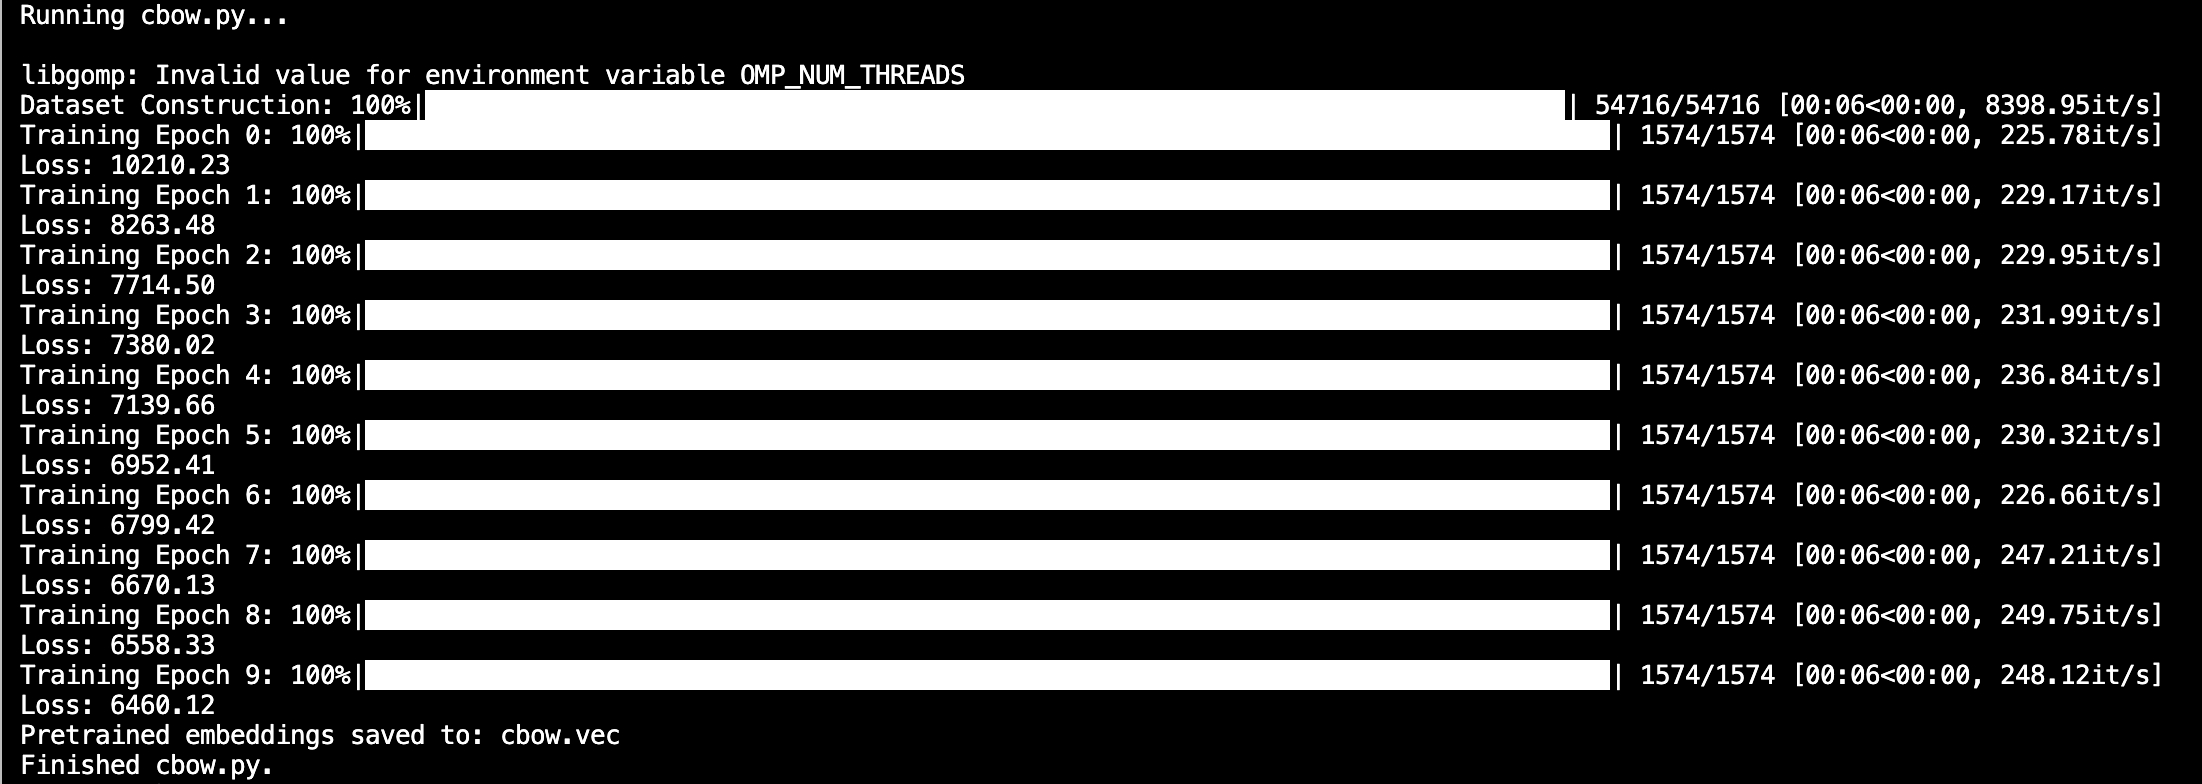
\includegraphics[width=0.78\textwidth]{embedding_model/cbow_training_log.jpeg}
    \caption{Training log screenshot for the CBOW model.}
    \label{fig:training-log-cbow}
\end{figure}

\begin{figure}[H]
    \centering
    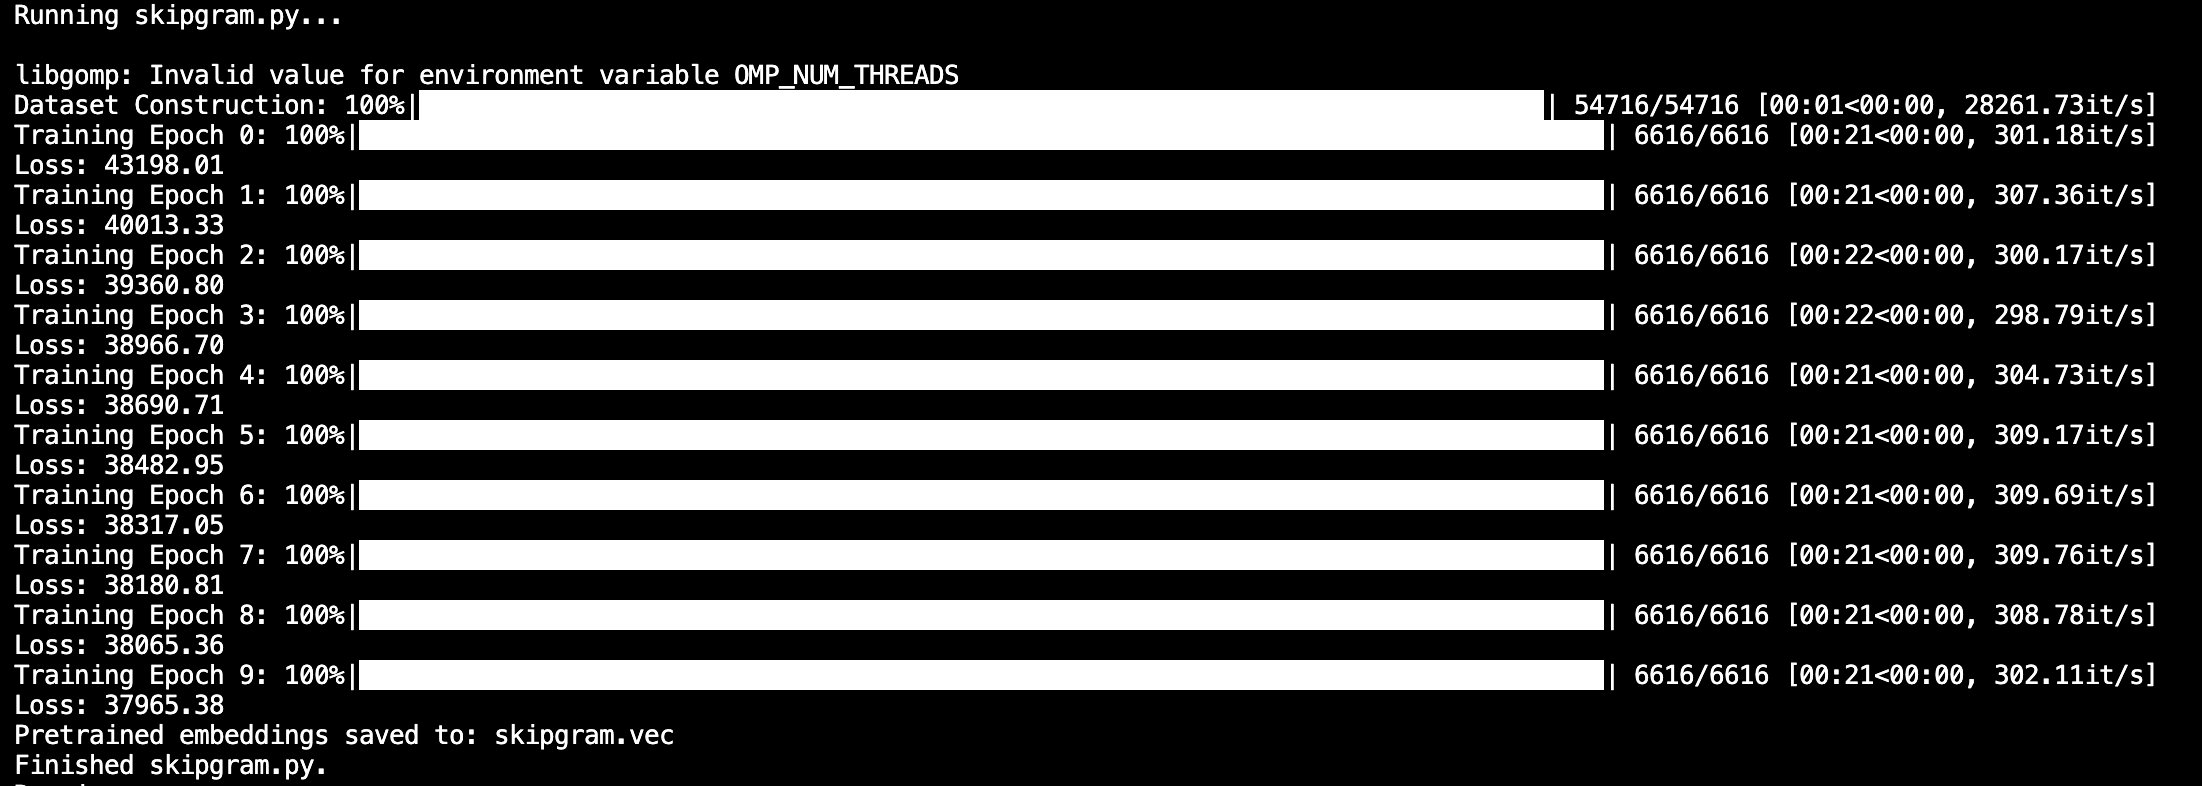
\includegraphics[width=0.78\textwidth]{embedding_model/skipgram_training_log.jpeg}
    \caption{Training log screenshot for the Skip-Gram model.}
    \label{fig:training-log-skipgram}
\end{figure}

\begin{figure}[H]
    \centering
    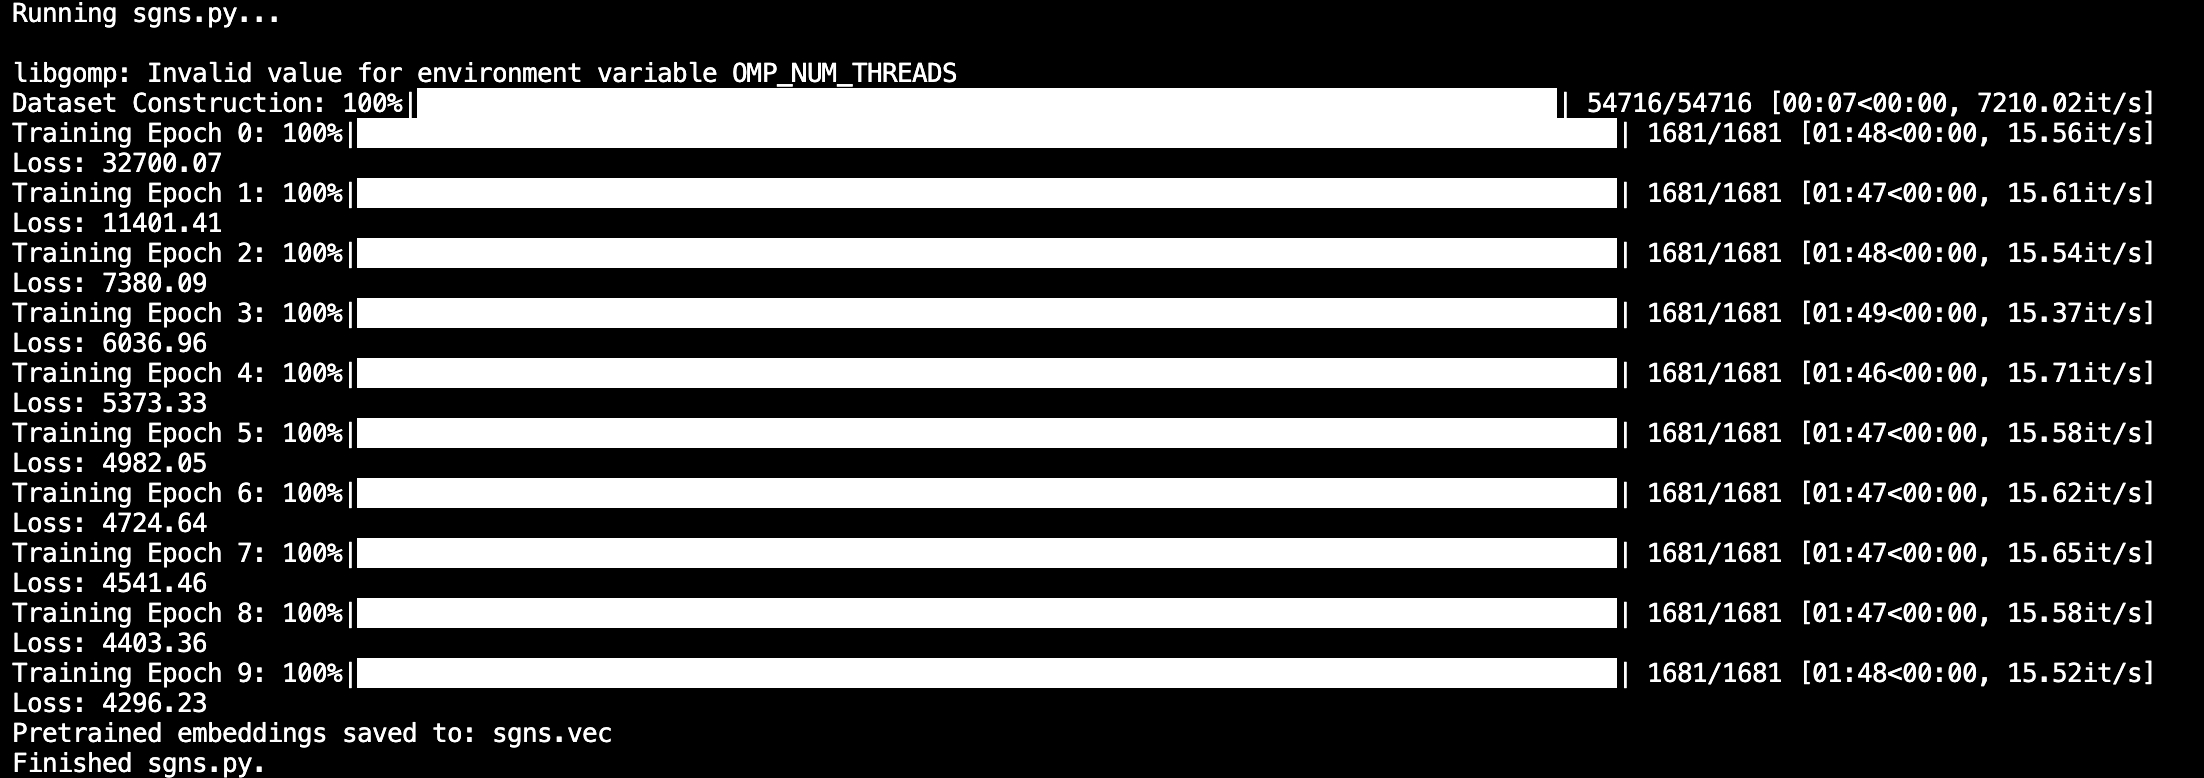
\includegraphics[width=0.78\textwidth]{embedding_model/sgns_training_log.jpeg}
    \caption{Training log screenshot for the SGNS model.}
    \label{fig:training-log-sgns}
\end{figure}

\section{Evaluation Methodology}
\subsection{KNN Evaluation}
For each of the 50 query words provided in the template, cosine similarity was used to retrieve the top 10 nearest neighbours from the embedding space. Following the project requirement, the mean similarity for each query was computed, and then an overall average similarity was computed across all valid query words. One query word (\texttt{realm}) was out of vocabulary in the current models, so the overall average was computed over 49 valid queries.

\subsection{SimLex-999 Evaluation}
The SimLex-999 benchmark contains manually annotated word pairs with gold similarity scores. For each pair, the cosine similarity between the two embeddings was computed and then scaled to the range $[0,10]$ using
\[
\text{scaled similarity} = (\cos(x,y) + 1) \times 5.
\]
The final model quality was measured by Spearman correlation between the gold scores and the embedding-based scores.

\subsection{Analogy Reasoning Evaluation}
For each analogy question in the form $A:B::C:D$, the predicted vector was computed as
\[
\mathbf{d}_{pred} = \mathbf{b} - \mathbf{a} + \mathbf{c}.
\]
The nearest embedding to $\mathbf{d}_{pred}$ was then selected, excluding the original words $A$, $B$, and $C$. Accuracy was measured as the number of exact matches among all valid analogy questions. In addition, ten sampled examples were printed for discussion, and five vector plots were generated for each model to satisfy the plotting requirement in the supplementary project PDF.

\section{Results}
\subsection{Overall Quantitative Results}
Table~\ref{tab:overall-results} summarizes the main quantitative outcomes from the three evaluation tasks. The primary comparison required by the assignment is between CBOW and Skip-Gram; the SGNS row is included only as additional context.

\begin{table}[H]
    \centering
    \caption{Overall results for the required CBOW and Skip-Gram models, with SGNS as an additional comparison.}
    \label{tab:overall-results}
    \begin{tabular}{lccc}
        \toprule
        Model & KNN overall avg. sim. & SimLex Spearman & Analogy correct / 8591 \\
        \midrule
        CBOW & 0.4928 & 0.0809 & 45 \\
        Skip-Gram & 0.5506 & 0.0818 & 60 \\
        SGNS & 0.5506 & 0.0423 & 19 \\
        \bottomrule
    \end{tabular}
\end{table}

Among the two required models, Skip-Gram achieved the strongest overall performance. It outperformed CBOW on all three evaluation tasks, although the SimLex-999 gap was small. The SGNS row is still informative as a supplementary reference: although SGNS matched Skip-Gram on the KNN average similarity metric, it was clearly weaker on SimLex-999 and especially on analogy reasoning.

\subsection{KNN Evaluation Results}
The KNN evaluation is intended to test whether semantically related words are placed close to one another in the learned embedding space. Following the project PDF, this section focuses on four shared query words so that the required CBOW and Skip-Gram models can be compared directly. The overall average similarity is 0.4928 for CBOW and 0.5506 for Skip-Gram, which already suggests that Skip-Gram forms tighter neighbourhoods on average.

\begin{table}[H]
    \centering
    \caption{KNN comparison for four shared query words in the required CBOW and Skip-Gram models.}
    \label{tab:knn-model-examples}
    \begin{tabular}{p{0.12\textwidth}p{0.14\textwidth}p{0.52\textwidth}}
        \toprule
        Query & Model & Representative nearest neighbours \\
        \midrule
        \texttt{july} & CBOW & june, april, march, october, december \\
        \texttt{july} & Skip-Gram & april, june, october, august, march \\
        \midrule
        \texttt{willing} & CBOW & trying, prepared, determined, going, needed \\
        \texttt{willing} & Skip-Gram & ready, needed, able, prepared, entitled \\
        \midrule
        \texttt{good} & CBOW & cautious, still, serious, brand, showing \\
        \texttt{good} & Skip-Gram & positive, addresses, favourable, flat, punch \\
        \midrule
        \texttt{very} & CBOW & penalty, serious, probably, still, pretty \\
        \texttt{very} & Skip-Gram & extremely, relatively, fairly, serious, strained \\
        \bottomrule
    \end{tabular}
\end{table}

\begin{figure}[H]
    \centering
    \begin{subfigure}[t]{0.48\textwidth}
        \centering
        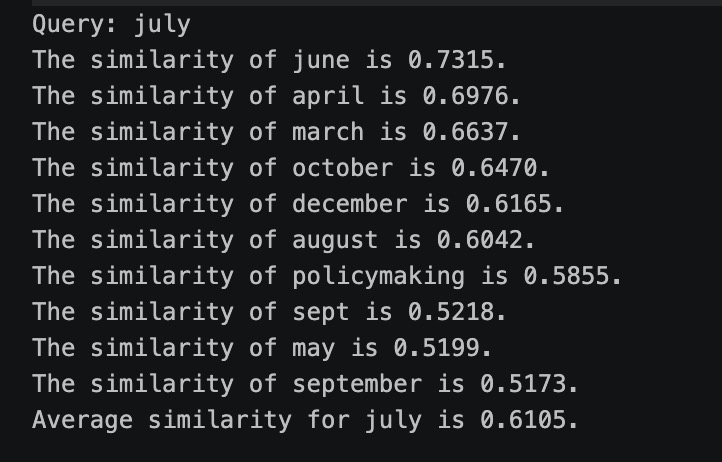
\includegraphics[width=\textwidth]{evaluation_results/cbow/cbow_knn_july.jpg}
        \caption{CBOW KNN example for \texttt{july}.}
    \end{subfigure}
    \hfill
    \begin{subfigure}[t]{0.48\textwidth}
        \centering
        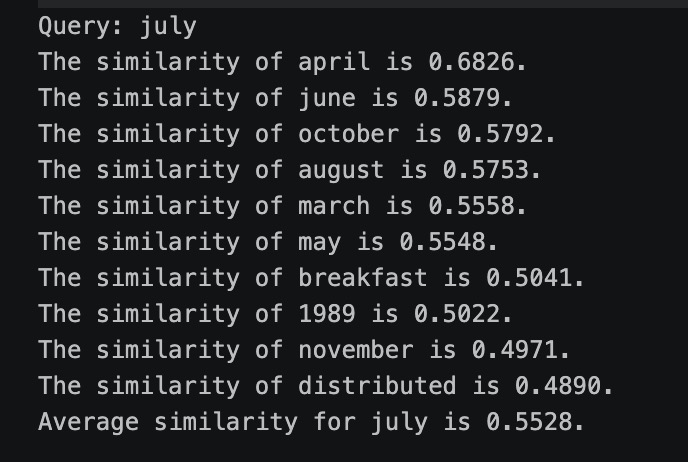
\includegraphics[width=\textwidth]{evaluation_results/skipgram/skipgram_knn_july.jpg}
        \caption{Skip-Gram KNN example for \texttt{july}.}
    \end{subfigure}
    \caption{Side-by-side KNN example figures for the shared query word \texttt{july}.}
    \label{fig:knn-july-comparison}
\end{figure}

Skip-Gram gives the clearer overall KNN behaviour on these four shared words. For \texttt{july}, both models recover a month cluster, but Skip-Gram is slightly cleaner because all top neighbours remain temporal words. For \texttt{willing}, the difference is more obvious: CBOW mixes plausible words with weaker items such as \texttt{going}, while Skip-Gram returns a more coherent readiness-related cluster headed by \texttt{ready}, \texttt{able}, and \texttt{prepared}. For \texttt{good}, both models still contain noisy neighbours, but Skip-Gram at least includes more clearly positive words such as \texttt{positive} and \texttt{favourable}. The strongest contrast appears for \texttt{very}: CBOW includes items like \texttt{penalty}, whereas Skip-Gram gives a much more convincing set of intensifiers such as \texttt{extremely}, \texttt{relatively}, and \texttt{fairly}. Overall, the shared-query comparison supports the quantitative result that Skip-Gram is better than CBOW on the required KNN evaluation.

\paragraph{Supplementary SGNS comparison.}
SGNS obtained the same overall average KNN similarity as Skip-Gram, but its qualitative behaviour was more mixed. For \texttt{july}, the top neighbours included \texttt{june}, \texttt{april}, \texttt{october}, \texttt{august}, and \texttt{september}, which is an excellent semantic grouping and stronger than the corresponding CBOW result. The query \texttt{very} also produced a coherent neighbourhood including \texttt{good}, \texttt{still}, \texttt{too}, and \texttt{much}, showing that SGNS can cluster high-frequency discourse words effectively. On the other hand, the query \texttt{company} returned words such as \texttt{parent}, \texttt{expects}, \texttt{said}, and \texttt{holding}; these are plausible in a news corpus but indicate topic or discourse association rather than pure semantic similarity. Therefore, SGNS appears to form tight contextual neighbourhoods, but these neighbourhoods are not always the most semantically precise.

\subsection{SimLex-999 Results}
The SimLex-999 evaluation measures how well the learned similarities align with expert judgments of semantic similarity. The overall Spearman correlation is 0.0809 for CBOW, 0.0818 for Skip-Gram, and 0.0423 for SGNS. Therefore, all three models perform weakly on this benchmark, but Skip-Gram is the strongest of the required models and SGNS is clearly worse. To show the pairwise behaviour behind these summary scores, Table~\ref{tab:simlex-samples} keeps 20 representative in-vocabulary pairs for the two required models and adds a simple judgement of whether each scaled similarity is broadly consistent with the gold-standard expectation.

In Table~\ref{tab:simlex-samples}, a result is marked as ``expected'' when the model score is broadly consistent with the SimLex gold score. Concretely, high-similarity pairs ($\text{gold} \geq 7$) are expected to receive high model scores ($\geq 5.5$), low-similarity pairs ($\text{gold} \leq 3$) are expected to receive low model scores ($\leq 4.5$), and mid-range pairs are marked as expected when the absolute difference between the model score and the gold score is no more than 2.0.

\begin{longtable}{p{0.16\textwidth}p{0.08\textwidth}p{0.09\textwidth}p{0.11\textwidth}p{0.11\textwidth}p{0.09\textwidth}}
    \caption{Twenty sampled SimLex-999 pairs for the required CBOW and Skip-Gram models.} \label{tab:simlex-samples} \\
    \toprule
    Word pair & Gold & CBOW & CBOW expected? & Skip-Gram & Skip-Gram expected? \\
    \midrule
    \endfirsthead
    \toprule
    Word pair & Gold & CBOW & CBOW expected? & Skip-Gram & Skip-Gram expected? \\
    \midrule
    \endhead
    \texttt{old -- new} & 1.58 & 6.82 & No & 6.57 & No \\
    \texttt{smart -- intelligent} & 9.20 & 4.65 & No & 5.38 & No \\
    \texttt{hard -- difficult} & 8.77 & 6.55 & Yes & 6.28 & Yes \\
    \texttt{hard -- easy} & 0.95 & 5.43 & No & 6.11 & No \\
    \texttt{fast -- rapid} & 8.75 & 6.01 & Yes & 5.94 & Yes \\
    \texttt{happy -- glad} & 9.17 & 6.60 & Yes & 5.90 & Yes \\
    \texttt{short -- long} & 1.23 & 8.06 & No & 7.67 & No \\
    \texttt{wide -- narrow} & 1.03 & 5.18 & No & 6.40 & No \\
    \texttt{bad -- awful} & 8.42 & 5.71 & Yes & 6.11 & Yes \\
    \texttt{easy -- difficult} & 0.58 & 6.05 & No & 7.06 & No \\
    \texttt{bad -- terrible} & 7.78 & 4.54 & No & 6.11 & Yes \\
    \texttt{insane -- crazy} & 9.57 & 5.08 & No & 5.26 & No \\
    \texttt{large -- huge} & 9.47 & 6.58 & Yes & 7.77 & Yes \\
    \texttt{quick -- rapid} & 9.70 & 6.55 & Yes & 5.02 & No \\
    \texttt{simple -- easy} & 9.40 & 5.54 & No & 6.08 & Yes \\
    \texttt{apparent -- obvious} & 8.47 & 5.68 & No & 5.99 & No \\
    \texttt{inexpensive -- cheap} & 8.72 & 6.24 & Yes & 5.47 & No \\
    \texttt{necessary -- important} & 7.37 & 7.37 & Yes & 6.48 & Yes \\
    \texttt{essential -- necessary} & 8.97 & 6.60 & Yes & 6.20 & Yes \\
    \texttt{crucial -- important} & 8.82 & 6.81 & Yes & 7.23 & Yes \\
    \bottomrule
\end{longtable}

\paragraph{Comment on the CBOW results.}
The CBOW results show a mixed pattern. It performs reasonably on some high-similarity pairs such as \texttt{hard -- difficult}, \texttt{fast -- rapid}, \texttt{large -- huge}, and \texttt{necessary -- important}, where the scaled similarities are at least directionally consistent with the gold scores. However, many clear mismatches remain. CBOW strongly overestimates contrastive pairs such as \texttt{old -- new}, \texttt{short -- long}, and \texttt{easy -- difficult}, while it underestimates strong synonym pairs such as \texttt{smart -- intelligent}, \texttt{insane -- crazy}, and \texttt{apparent -- obvious}. This suggests that CBOW captures broad relatedness better than precise semantic similarity.

\paragraph{Comment on the Skip-Gram results.}
Skip-Gram shows a very similar overall pattern, but it is slightly better on several representative pairs. It gives more plausible scores for \texttt{bad -- terrible}, \texttt{large -- huge}, \texttt{simple -- easy}, and \texttt{crucial -- important}, and this is consistent with its slightly higher Spearman score. At the same time, it still makes many of the same mistakes as CBOW. For example, \texttt{hard -- easy}, \texttt{short -- long}, and \texttt{wide -- narrow} are all scored much too highly, while \texttt{smart -- intelligent} and \texttt{apparent -- obvious} are still underestimated. Therefore, Skip-Gram is somewhat stronger, but it does not solve the core limitation of confusing relatedness with similarity.

\paragraph{Performance comparison between CBOW and Skip-Gram.}
Comparing the two required models, Skip-Gram has a small but real advantage overall. It handles several important synonym-like pairs better and achieves the best final Spearman correlation, even if the margin over CBOW is small. CBOW is still competitive and is actually closer on some pairs such as \texttt{quick -- rapid} and \texttt{inexpensive -- cheap}. Nevertheless, when the 20 sampled pairs are viewed together with the final correlation scores, Skip-Gram gives the more reliable SimLex-999 behaviour in this project, while both models remain far from human-level semantic judgement.

\subsection{Analogy Reasoning Results}
Analogy reasoning was the most difficult task among the three evaluations. In total, there are 8591 valid analogy questions whose four words all appear in the vocabulary. Among the two required models, CBOW correctly answered 45 of these 8591 questions, while Skip-Gram correctly answered 60. For completeness, SGNS correctly answered 19. Therefore, all three models show very low overall analogy accuracy, although Skip-Gram is the strongest of the required models.

The project PDF also asks for sampled analogy outputs and vector plots rather than only a final accuracy. The saved result files already contain 10 sampled examples for each required model. To keep the presentation concise, Tables~\ref{tab:analogy-cbow-samples} and \ref{tab:analogy-skipgram-samples} each show 5 representative examples from the saved outputs.

\begin{table}[H]
    \centering
    \caption{Five sampled analogy results from the saved CBOW outputs.}
    \label{tab:analogy-cbow-samples}
    \begin{tabular}{p{0.34\textwidth}p{0.14\textwidth}p{0.14\textwidth}p{0.12\textwidth}}
        \toprule
        Analogy & Expected & CBOW pred. & Correct? \\
        \midrule
        \texttt{shrinking:shrank::taking:?} & \texttt{took} & \texttt{took} & Yes \\
        \texttt{seattle:washington::baltimore:?} & \texttt{maryland} & \texttt{dyr} & No \\
        \texttt{athens:greece::helsinki:?} & \texttt{finland} & \texttt{threatened} & No \\
        \texttt{old:older::big:?} & \texttt{bigger} & \texttt{themselves} & No \\
        \texttt{cheap:cheaper::cool:?} & \texttt{cooler} & \texttt{fo} & No \\
        \bottomrule
    \end{tabular}
\end{table}

\begin{table}[H]
    \centering
    \caption{Five sampled analogy results from the saved Skip-Gram outputs.}
    \label{tab:analogy-skipgram-samples}
    \begin{tabular}{p{0.34\textwidth}p{0.14\textwidth}p{0.14\textwidth}p{0.12\textwidth}}
        \toprule
        Analogy & Expected & Skip-Gram pred. & Correct? \\
        \midrule
        \texttt{australia:australian::germany:?} & \texttt{german} & \texttt{german} & Yes \\
        \texttt{seattle:washington::baltimore:?} & \texttt{maryland} & \texttt{nuts} & No \\
        \texttt{athens:greece::helsinki:?} & \texttt{finland} & \texttt{rinn} & No \\
        \texttt{old:older::big:?} & \texttt{bigger} & \texttt{corproration} & No \\
        \texttt{cheap:cheaper::cool:?} & \texttt{cooler} & \texttt{toepfer} & No \\
        \bottomrule
    \end{tabular}
\end{table}

For visualization, one representative vector plot is shown for each required model. Figure~\ref{fig:analogy-cbow-correct} shows a correct CBOW example, while Figure~\ref{fig:analogy-skipgram-correct} shows a correct Skip-Gram example.

\begin{figure}[H]
    \centering
    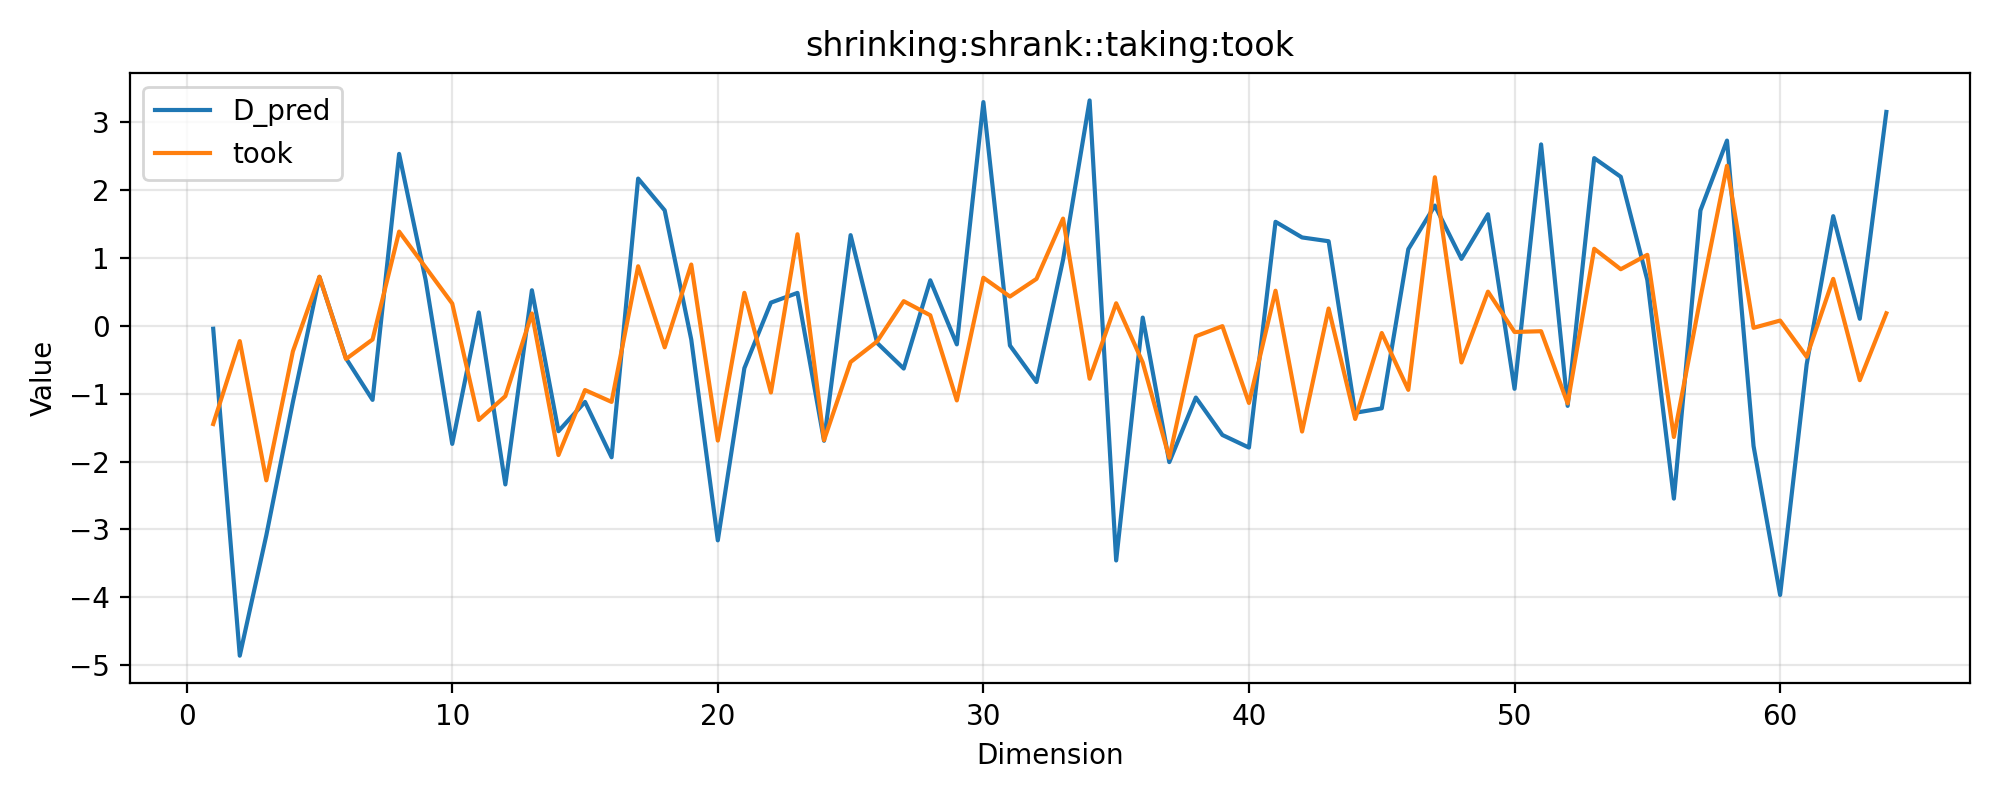
\includegraphics[width=0.78\textwidth]{evaluation_results/cbow/analogy_plots/01_shrinking_shrank_taking_took.png}
    \caption{CBOW plot for the correct example \texttt{shrinking : shrank :: taking : took}.}
    \label{fig:analogy-cbow-correct}
\end{figure}

\begin{figure}[H]
    \centering
    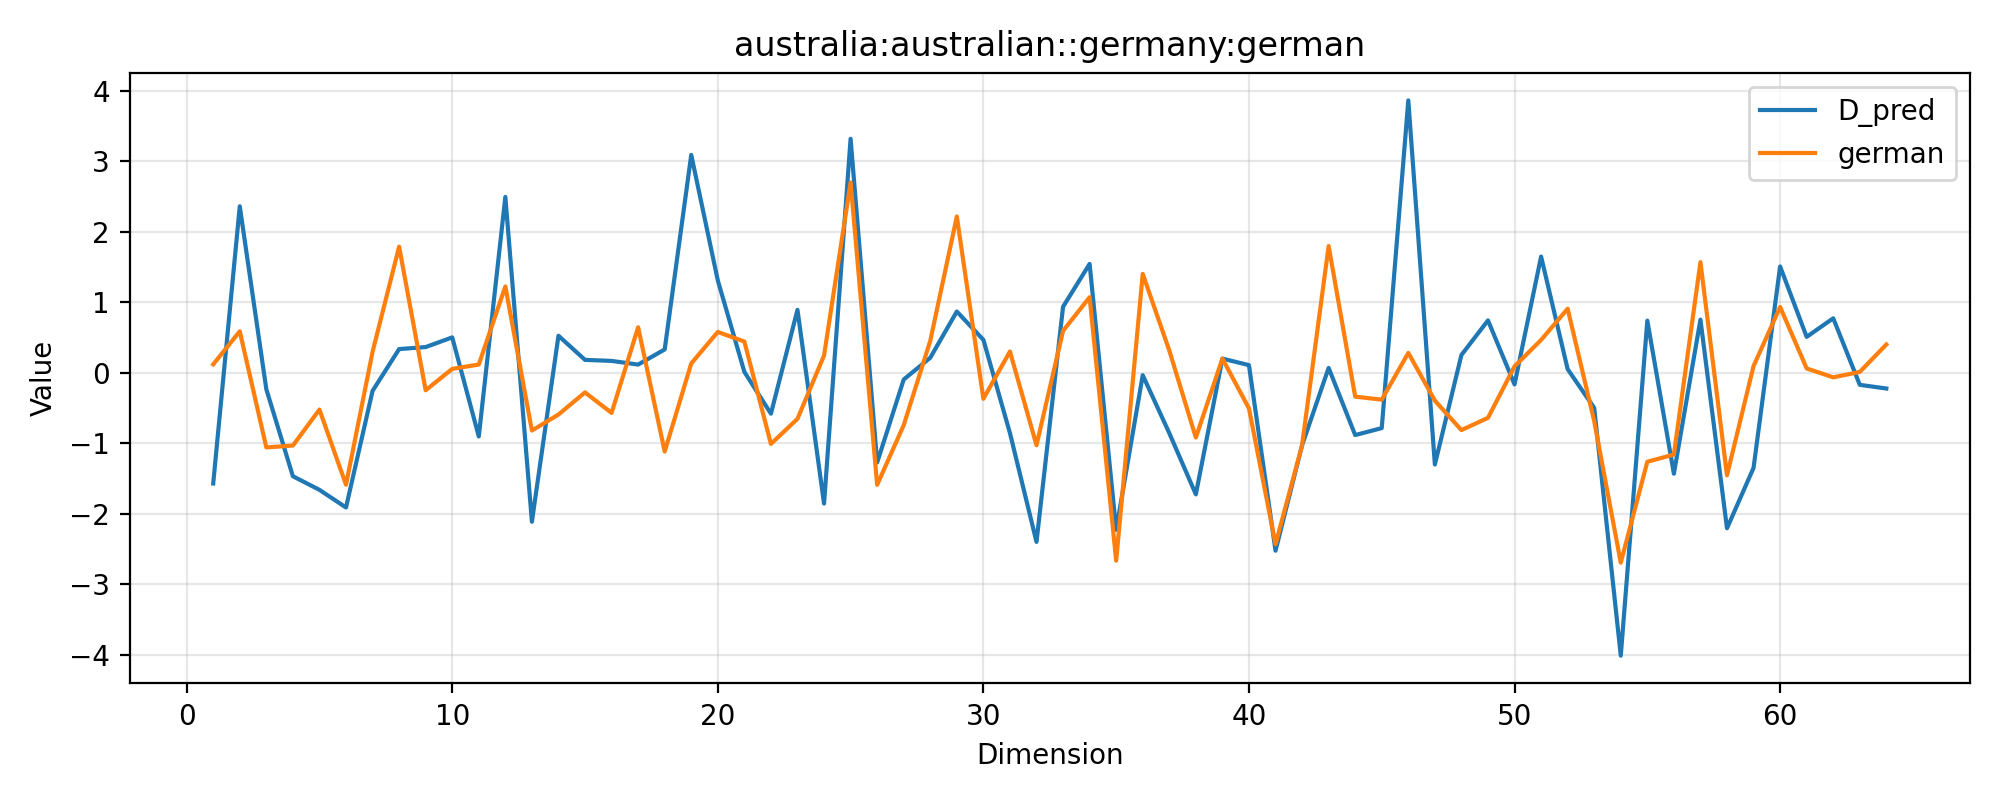
\includegraphics[width=0.78\textwidth]{evaluation_results/skipgram/analogy_plots/01_australia_australian_germany_german.png}
    \caption{Skip-Gram plot for the correct example \texttt{australia : australian :: germany : german}.}
    \label{fig:analogy-skipgram-correct}
\end{figure}

The two sample tables show the same overall pattern as the full accuracy scores. Each model can occasionally solve a clean morphological or nationality relation, but most predictions are clearly wrong and often collapse to unrelated words. This suggests that the analogy vector $\mathbf{b}-\mathbf{a}+\mathbf{c}$ is usually not landing near a stable semantic relation in the learned space. One likely reason is that the embeddings were trained on a relatively noisy corpus with many rare tokens, misspellings, and corpus-specific names, so the neighbourhood around the predicted vector is easily dominated by accidental co-occurrence patterns instead of genuine relational structure. A second reason is that analogy reasoning is a much stricter test than KNN or word similarity: it requires not only that similar words be close, but also that specific linear offsets such as country$\rightarrow$capital, adjective$\rightarrow$comparative, or nation$\rightarrow$nationality be represented consistently across many examples. The sampled errors show that this consistency is weak here. For instance, instead of returning state or country names, the models produce tokens such as \texttt{dyr}, \texttt{rinn}, \texttt{nuts}, and \texttt{communications}, which suggests that the nearest-neighbour search is being pulled toward noisy local clusters rather than meaningful relation-specific answers. Even the comparative examples fail in this way: \texttt{bigger} and \texttt{cooler} are replaced by unrelated items such as \texttt{themselves}, \texttt{corproration}, \texttt{fo}, and \texttt{toepfer}. Overall, Skip-Gram is still slightly better than CBOW because its total accuracy is higher and it preserves a few relations more clearly, but both models remain weak on analogy reasoning because the embedding space is not regular enough to support robust vector arithmetic.

\section{Discussion}
Several conclusions can be drawn from the results. First, among the two required models, Skip-Gram was the stronger overall choice in this project. It achieved a higher KNN average similarity than CBOW, a slightly higher SimLex-999 Spearman correlation, and a clearly better analogy accuracy. Taken together, these results suggest that Skip-Gram learned a more useful embedding geometry for both local similarity and relational reasoning.

Second, CBOW still showed some meaningful behaviour, especially for broad semantic classes such as months and for a small number of successful morphology-based analogies. However, compared with Skip-Gram, its KNN results were less consistently interpretable and its analogy performance was weaker. This suggests that the CBOW vectors were less sharply organized for the evaluation tasks required in the project PDF.

Third, the supplementary SGNS comparison helps interpret the required results more carefully. Although SGNS matched Skip-Gram on the KNN average similarity metric, it was clearly worse on SimLex-999 and analogy reasoning. This suggests that high local cosine similarity alone is not enough to guarantee semantically precise or relationally useful embeddings.

Finally, the overall scores also reveal a broader limitation of the training setup. Many outputs include noisy tokens, misspellings, or rare corpus-specific words. This likely reflects limitations in preprocessing and corpus quality rather than only model design. In other words, the embedding quality depends not only on the neural architecture, but also on vocabulary filtering, corpus coverage, and token cleanliness.

\section{Conclusion}
This project implemented and evaluated the two required Word2Vec models, CBOW and Skip-Gram, using the three evaluation tasks specified in the project documents: KNN evaluation, SimLex-999 evaluation, and analogy reasoning evaluation. An additional SGNS comparison was also included as a supplementary extension.

Across the required models, Skip-Gram performed best overall. It produced more convincing nearest neighbours than CBOW, achieved a slightly better SimLex-999 correlation, and gave the strongest analogy accuracy. Even so, both required models still showed clear limitations in semantic precision and relational reasoning, especially on SimLex-999 and large-scale analogy evaluation.

Overall, the report provides the required training evidence, applies all three evaluation methods to both CBOW and Skip-Gram vectors, and compares the resulting behaviour through quantitative summaries, selected qualitative examples, and vector plots. Future improvements could include stronger preprocessing, better vocabulary cleaning, hyperparameter tuning, and training on a larger or cleaner corpus. These changes may improve both the interpretability of nearest neighbours and the consistency of analogy reasoning.

\end{document}
